%! Author = antonio
%! Date = 7/2/24

Before proceeding with classification, two techniques of dimensionality reduction PCA and LDA can be analysed.
The goal is to find a subspace of the feature space that preserves most of the useful information, that is, mapping from
the \(n\text{–}dimensional\) feature space to \(m\text{–}dimensional\) space, with
\(m \ll n\)

% PCA

\subsection{PCA}
\label{subsec:pca} is an unsupervised technique.
Where starting from a dataset \(X = \{x_1, \dots,x_k\}\) and calculated average.
It starts with the empirical covariance matrix:
\begin{equation}
    C = \frac{1}{K} \sum (x_i - \bar{x})(x_i - \bar{x})^T
    \label{eq:covarianceMatrix}
\end{equation}

We compute the eigen-decomposition of \(C = U \Sigma U^T\) and project the data in the subspace
spanned by the \(m\) columns of \(U\) corresponding to the \(m\) largest eigenvalues.
\begin{equation}
    y_i = P^T(x_i - \bar{x})
    \label{eq:projection}
\end{equation}

where P is the matrix of the \(m\) columns of U associated to the m highest eigenvalues of \(C\).
A cross-validation approach can be used to figure out the optimal value of m to be selected.
To evaluate each eigenvalue, one would have to calculate the variance corresponding to the axis.
The percentage can be calculated as the rate between the sum of the m eigenvalues and the sum of all of them.
In \autoref{fig:percentageVariance} we can see how it changes in the project.
A good m, corresponds to that value which allows a percentage greater than 95\%, so in our case we would need all 6
features.

\begin{figure}[h!]
    \centering
    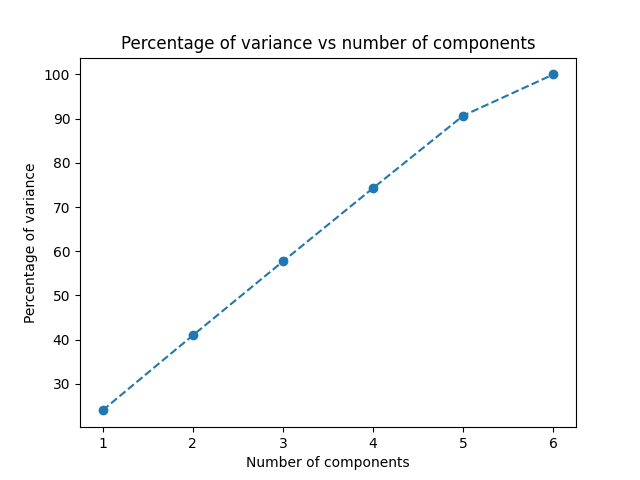
\includegraphics[width=0.5\linewidth]{Lab/03. Lab 03/Images/01. PercentageVariance_NumberOfComponents}
    \caption{Cross validation for PCA impact evaluation}
    \label{fig:percentageVariance}
\end{figure}

% LDA

\subsection{LDA}
\label{subsec:LDA} is a supervised technique.
To find a direction that has the best separation between classes, we measure spread between classes in terms of class covariance.
The objective is to maximize the \(between-class\) variability over \(within-class\) variability ratio for the transformed samples:
\begin{equation}
    \underset{w}{\max} \frac{w^T S_B w}{w^T S_W w}
    \label{eq:ldaFunct}
\end{equation}

where:
\begin{equation}
    S_B  \triangleq \frac{1}{N}\sum_{c=1}^{K} n_c (\mu_c - \mu)(\mu_c - \mu)^T
    \label{eq:betweenClass}
\end{equation}

\begin{equation}
    S_W \triangleq \frac{1}{N}\sum_{c=1}^{K} \sum_{i=1}^{n_c} (x_{c,i} - \mu_c)(x_{c,i} - \mu_c)^T
    \label{eq:withinClass}
\end{equation}

\(\mu\) is dataset mean
\(\mu_{c}\) is class mean

% OUR PROJECT

\subsection{Our project}
\label{subsec:ourProject}
PCA and LDA are applied to the dataset, in particular, m = 6 is used, and in \autoref{fig:pcaLda} we can observe
what are the outcomes for the indicated directions.

\begin{figure}[h]
    \centering
    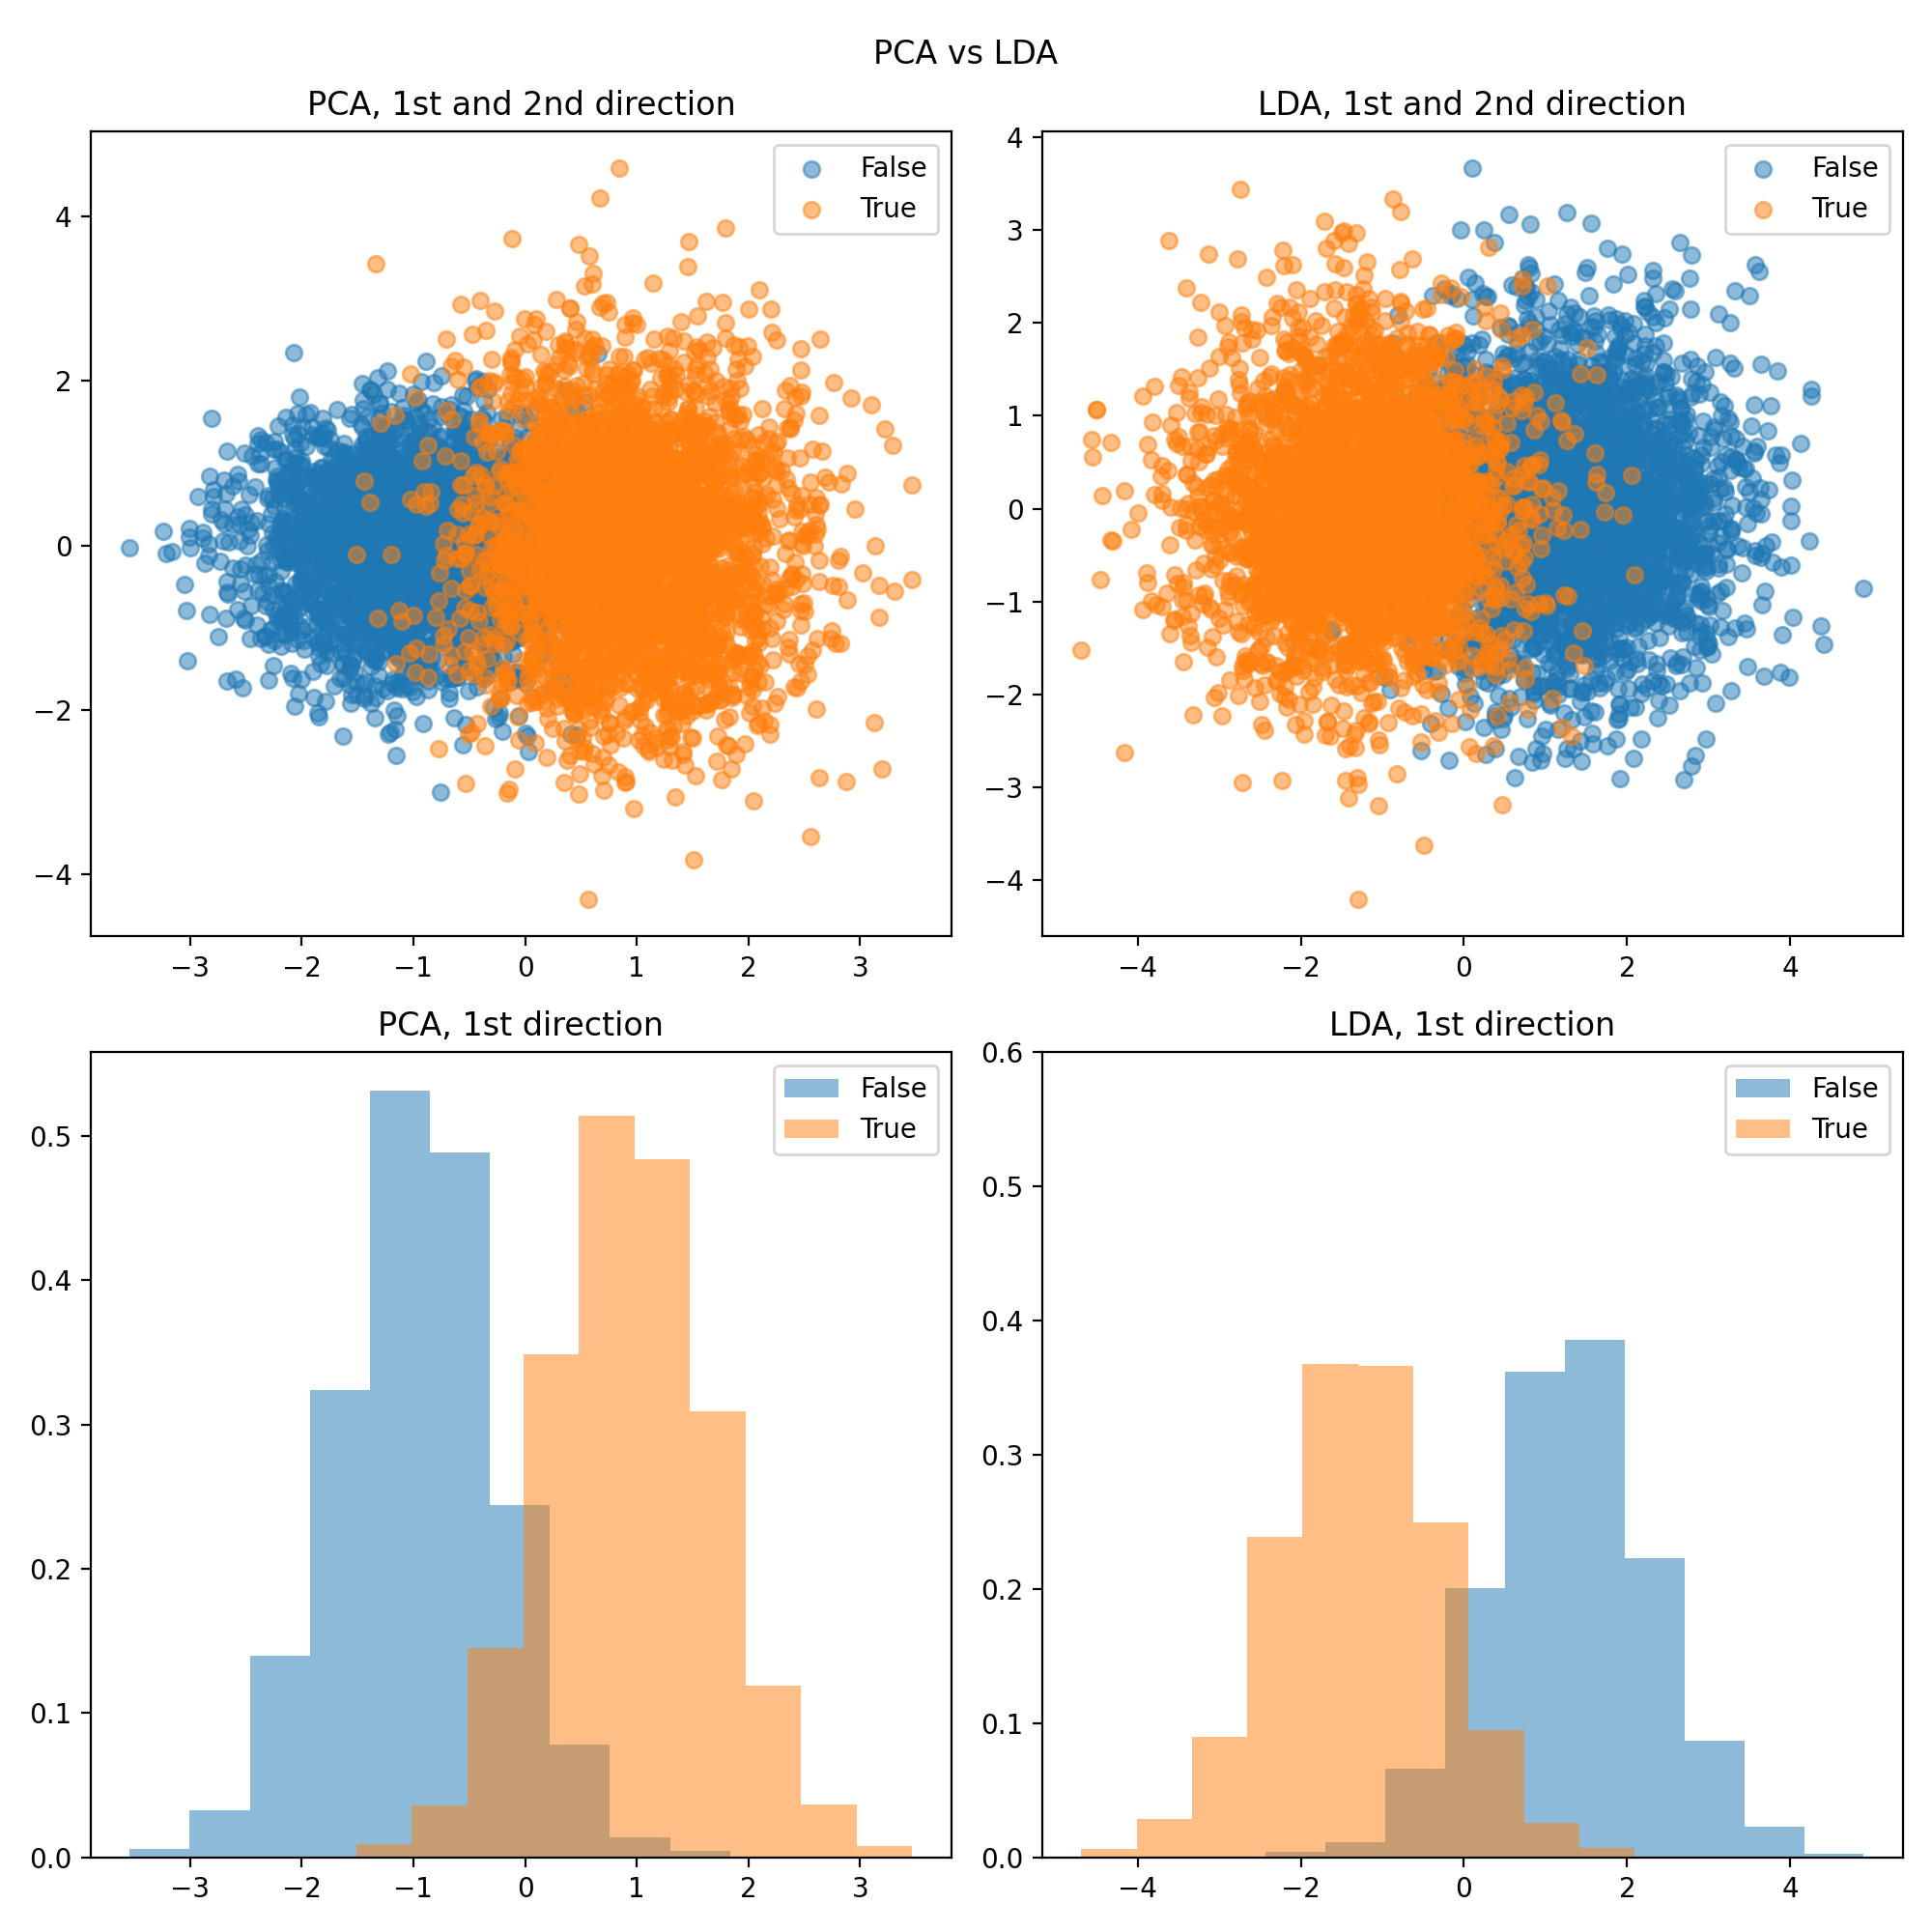
\includegraphics[width=0.5\linewidth]{Lab/03. Lab 03/Images/02. PVA_LDA}
    \caption{Comparing resulta between PCA and LDA}
    \label{fig:pcaLda}
\end{figure}

At a later stage, they were used to carry out a classification.
The available dataset was divided into two sub-portions one for training and the other for validation.
In \autoref{tab:LDAPCAForClassification} we can see the error of the classification,
errors made in the classification when varying m (only for some values) and the threshold were reported

\begin{table}
    \centering
    \begin{tabular}{c c c c}
        \toprule
        \textbf{Method}                    & \textbf{Num Samples} & \textbf{Error} & \textbf{Error Rate} (\%) \\
        \midrule
        LDA - First threshold              & 2000                 & 186            & 9.30                     \\
        LDA - Second threshold             & 2000                 & 186            & 9.30                     \\
        \midrule
        PCA (m=5) + LDA - First threshold  & 2000                 & 186            & 9.30                     \\
        PCA (m=5) + LDA - Second threshold & 2000                 & 185            & 9.25                     \\
        PCA (m=6) + LDA - First threshold  & 2000                 & 186            & 9.30                     \\
        PCA (m=6) + LDA - Second threshold & 2000                 & 184            & 9.20                     \\
        \bottomrule
    \end{tabular}
    \captionsetup{justification=justified,singlelinecheck=false,format=hang}
    \caption{Table showing the results of the LDA and PCA + LDA method for classification.}
    \label{tab:LDAPCAForClassification}
\end{table}








